

\section{\trDisplacementEnergy{}与\trCapacity{}之间的不等式}
\label{sec:displacement-inequality}

\hzsync{theorem}{5}%
\hzsync{proposition}{14}%
\hzsync{lemma}{7}%
\hzsync{corollary}{2}%
\hzsync{definition}{5}%
\hzsync{equation}{24}%
\hzsync{figure}{2}%

\trEnergy{}函数 $E:\mathcal{D}\to\R^{+}$ 定义为
\[
E(\psi)=\inf\bigl\{\,\lVert H\rVert\ \bigm|\ \psi=\varphi_{H}\,\bigr\},
\]
其中 $H\in\mathcal{H}$，并且采用记号 $H_{t}(x)=H(t,x)$，
\[
\lVert H\rVert=\int_{0}^{1}\Bigl(\sup_{x}H_{t}-\inf_{x}H_{t}\Bigr)\,dt.
\]

\trEnergy{}与\trCapacity{}之间的关系如前文所述，我们将证明

\begin{theorem}\label{thm:energy-dominates-capacity}
若 $\psi\in\mathcal{D}$，则
\[
E(\psi)\ \geq\ \sup\bigl\{\,c_{0}(U)\ \bigm|\ U\ \text{开且}\ \psi(U)\cap U=\varnothing\,\bigr\}.
\]
\end{theorem}

这里的 $c_{0}(U)$ 是第 3 章中引入的那个特殊\trCapacity。为了证明这个定理，%
我们将分若干步骤进行，先定义正、负\trEnergy{}函数 $E^{\pm}:\mathcal{D}\to\R^{+}$ 如下：
\begin{align*}
E^{+}(\psi)\ &=\ \inf\bigl\{\ \int_{0}^{1}\sup_{x}H_{t}\ dt\ \bigm|\ \psi=\varphi_{H}\bigr\}\\
E^{-}(\psi)\ &=\ -\sup\bigl\{\ \int_{0}^{1}\inf_{x}H_{t}\ dt\ \bigm|\ \psi=\varphi_{H}\bigr\}%
\ =\ \inf\bigl\{\ \int_{0}^{1}-\inf_{x}H_{t}\,dt\ \bigm|\ \psi=\varphi_{H}\bigr\}.
\end{align*}
显然，
\begin{align*}
E^{+}(\psi)+E^{-}(\psi)\ &\leq\ E(\psi)\\
E^{+}(\psi)\ &=\ E^{-}\bigl(\psi^{-1}\bigr).
\end{align*}

\begin{proposition}\label{prop:gamma-energy-estimate}
若 $\varphi,\psi\in\mathcal{D}$，则
\[
\gamma(\varphi)-E^{+}(\psi)\leq\gamma(\varphi\circ\psi)\leq\gamma(\varphi)+E^{-}(\psi).
\]
\end{proposition}

令 $\varphi=\id$，特别地，利用 $E^{+}(\psi)=E^{-}\bigl(\psi^{-1}\bigr)$ 便得
\[
E(\psi)\ \geq\ \gamma(\psi)+\gamma\bigl(\psi^{-1}\bigr).
\]

\begin{proof}
令 $\varphi=\varphi_{H}$ 与 $\psi=\varphi_{K}$，则 $\varphi\circ\psi=\varphi_{H\#K}$，%
于是
\begin{align*}
\gamma(\varphi\circ\psi)\ &=\ \sup_{F\in\mathcal{F}}\ \inf\ a_{H\#K}(F)\\
&=\ \sup_{F\in\mathcal{F}}\ \inf_{x\in F}\Bigl[a_{H}(x)-\int_{0}^{1}K_{t}\Bigl(\bigl(\varphi_{H}^{t}\bigr)^{-1}(x)\Bigr)\,dt\Bigr]\\
&\geq\ \gamma(\varphi)-\int_{0}^{1}\sup_{x}K_{t}\,dt
\end{align*}
这就蕴含了第一个不等式；第二个不等式可以类似地证明。
\end{proof}

\begin{lemma}\label{lem:gamma-invariance-disjoint}
设 $U\subset\R^{2n}$ 开且\trBounded，并设 $\varphi,\psi\in\mathcal{D}$ 满足
\begin{align*}
\text{(i)}\qquad& \varphi=\varphi_{H},\qquad\text{其中}\ \operatorname{supp}(H)\subset[0,1]\times U.\\
\text{(ii)}\qquad& \psi(U)\cap U=\varnothing.
\end{align*}
则
\[
\gamma(\varphi\circ\psi)=\gamma(\psi\circ\varphi)=\gamma(\psi).
\]
\end{lemma}

\begin{proof}
以 $\varphi_{\tau}=\varphi_{H}^{\tau}$ 记 $H$ 的\trFlow，我们有%
$\operatorname{Fix}(\varphi_{\tau}\circ\psi)=\operatorname{Fix}(\psi\circ\varphi_{\tau})=%
\operatorname{Fix}(\psi)\subset\R^{2n}\setminus U$。若 $\sigma$ 表示\trActionSpectrum，%
则我们断言
\begin{equation}\label{eq:sigma-invariance}
\sigma(\varphi_{\tau}\circ\psi)=\sigma(\psi)=\sigma(\psi\circ\varphi_{\tau}),
\end{equation}
对 $0\leq\tau\leq1$ 成立。的确，固定 $\tau$，通过对时间作\trReparametrization，%
我们可以选取新的\trHamiltonianFunction，即生成 $\psi$ 的 $K$ 与生成 $\varphi_{\tau}$ 的%
$H_{\tau}$，使得当 $\frac{1}{2}\leq t\leq1$ 时 $K(t,x)=0$，当 $0\leq t\leq\frac{1}{2}$ 时%
$H_{\tau}(t,x)=0$，且 $\operatorname{supp}(H_{\tau})\subset[0,1]\times U$。对相应的\trFlow，%
我们看到
\[
\psi^{t}\circ\varphi_{\tau}^{t}(x)=\psi^{t}(x)=\varphi_{\tau}^{t}\circ\psi^{t}(x),%
\qquad x\in\operatorname{Fix}(\psi),
\]
对一切 $0\leq t\leq1$ 成立，这就蕴含了 \eqref{eq:sigma-invariance}。函数%
$\tau\mapsto\gamma(\psi\circ\varphi_{\tau})$ 与 $\tau\mapsto\gamma(\varphi_{\tau}\circ\psi)$%
连续且取值于\trNowhereDense{}集 $\sigma(\psi)$ 之中，故必为常值，从而由%
$\varphi_{0}=\id$ 可知它们等于 $\gamma(\psi)$，引理得证。
\end{proof}

该\trhLemma{}的下述直接推论，对\cref{thm:energy-dominates-capacity}的证明将%
是至关重要的。

\begin{proposition}\label{prop:gamma-le-energy}
设 $\varphi,\psi\in\mathcal{D}$ 满足\cref{lem:gamma-invariance-disjoint}的假设，%
即存在一个开的有界子集 $U\subset\R^{2n}$，使得 $\varphi=\varphi_{H}$（%
$\operatorname{supp}(H)\subset[0,1]\times U$）且 $\psi(U)\cap U=\varnothing$。则
\[
\gamma(\varphi)\ \leq\ E(\psi).
\]
\end{proposition}

\begin{proof}
由\cref{lem:gamma-invariance-disjoint}知 $\gamma(\psi)=\gamma(\varphi\circ\psi)$；%
再由\cref{prop:gamma-energy-estimate}可得
\[
E^{-}(\psi)\ \geq\ \gamma(\psi)=\gamma(\varphi\circ\psi)\ \geq\ \gamma(\varphi)-E^{+}(\psi)
\]
从而 $\gamma(\varphi)\leq E^{+}(\psi)+E^{-}(\psi)\leq E(\psi)$，正是所要证的。
\end{proof}

对 $\mathcal{D}$ 中那些由特殊的不依赖时间的\trHamiltonianFunction{}所生成的%
$\psi$，我们有可能把\trEnergy{} $E(\psi)$ 与 $\gamma(\psi)$ 计算出来。

\begin{proposition}\label{prop:time-independent-energy}
设 $H\in\mathcal{H}$ 不依赖于时间，并且进一步设 $\dot{x}=X_{H}(x)$ 的一切满足%
$0<T\leq1$ 的 $T$-\trPeriodicSolution{}都是常值的。则对 $\varphi=\varphi_{H}$，
\begin{align*}
\gamma(\varphi)\ &=\ -\inf_{x}H\\
E(\varphi)\ &=\ \lVert H\rVert=\sup_{x}H-\inf_{x}H\\
E(\varphi)\ &=\ \gamma(\varphi)+\gamma\bigl(\varphi^{-1}\bigr).
\end{align*}
\end{proposition}

\begin{proof}
简记 $\varphi^{s}=\varphi_{H}^{s}$（$0\leq s\leq1$）。由关于诸\trPeriodicSolution{}的%
假设可知，$\varphi^{s}$ 的诸\trFixedPoint{}正是 $H$ 的诸\trCriticalPoint，从而
\[
\sigma\bigl(\varphi^{s}\bigr)=\bigl\{-sH(m)\ \bigm|\ dH(m)=0\bigr\}.
\]
简记负\trCritical{}水平之集为 $C_{H}=-\{H(m)\mid dH(m)=0\}$，我们便得出%
$\gamma\bigl(\varphi^{s}\bigr)\in sC_{H}$。据\trSard{}定理，$C_{H}$ 是\trNowhereDense{}的，%
而由于 $s\mapsto\frac{1}{s}\gamma\bigl(\varphi^{s}\bigr)\in C_{H}$ 是连续的，故它必为%
常值。于是，存在 $H$ 的一个\trCriticalPoint{} $m^{*}$，使得
\begin{equation}\label{eq:gamma-autonomous}
\gamma\bigl(\varphi^{s}\bigr)=-sH\bigl(m^{*}\bigr),\qquad\text{对一切}\ 0\leq s\leq1.
\end{equation}
我们将证明 $H\bigl(m^{*}\bigr)=\inf H$。仿照\cref{prop:gamma-h-properties}证明中的%
做法平移 $H$，我们可以假设 $H(0)=\inf H$。
据\cref{prop:gamma-energy-estimate}，
\[
\gamma\bigl(\varphi^{s}\bigr)=\gamma\bigl(\varphi_{sH}\bigr)\leq E^{-}\bigl(\varphi_{sH}\bigr)%
\leq-sH(0).
\]
另一方面，我们可以找到 $s_{0}>0$，使得 $sH(x)\leq sH(0)+\pi\lvert x\rvert^{2}$ 对一切%
$0\leq s\leq s_{0}$ 与 $x\in\R^{2n}$ 成立，这就蕴含
\begin{align*}
\gamma\bigl(\varphi_{sH}\bigr)\ &\geq\ \inf_{x\in E^{+}}\Bigl[a(x)-\pi\int_{0}^{1}\lvert x\rvert^{2}\Bigr]-sH(0)\\
&=\ -sH(0)
\end{align*}
于是 $\gamma\bigl(\varphi_{sH}\bigr)=-sH(0)$ 对一切 $0\leq s\leq s_{0}$ 成立，从而据%
\eqref{eq:gamma-autonomous}，对一切 $0\leq s\leq1$ 亦成立。我们便见到
\[
\gamma(\varphi)=-\inf H
\]
正是所要证的。现在 $\varphi_{-H}=\bigl(\varphi_{H}\bigr)^{-1}$，同一论证给出
\[
\gamma\bigl(\varphi^{-1}\bigr)=\gamma\bigl(\varphi_{-H}\bigr)=-\inf(-H)=\sup H.
\]
于是再由\cref{prop:gamma-energy-estimate}，
\begin{align*}
-\inf H\ &=\ \gamma(\varphi)\leq E^{-}(\varphi)\\
\sup H\ &=\ \gamma\bigl(\varphi^{-1}\bigr)\leq E^{-}\bigl(\varphi^{-1}\bigr)=E^{+}(\varphi).
\end{align*}
相加得
\[
\lVert H\rVert=\sup H-\inf H\leq E^{-}(\varphi)+E^{+}(\varphi)\leq E\bigl(\varphi_{H}\bigr)%
\leq\lVert H\rVert,
\]
故 $E(\varphi)=\lVert H\rVert$，正是所要证的。
\end{proof}

\noindent\begin{minipage}{\linewidth}
\centering
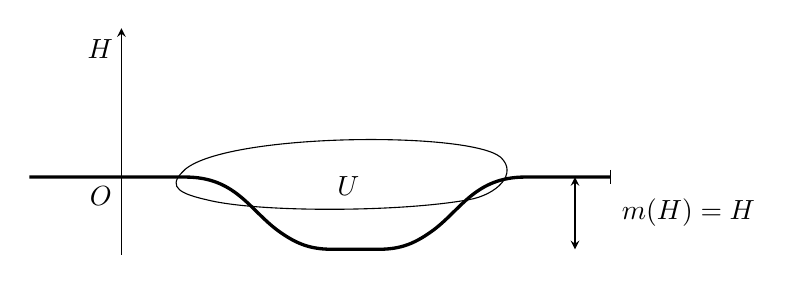
\begin{tikzpicture}[>=stealth,scale=0.9]
  \draw[->] (0,-1.1) -- (0,2.1);%
  \node at (-0.3,1.8) {$H$};
  \node[below left] at (0,0) {$O$};
  \draw[very thick] (-1.3,0) -- (0.9,0)
        .. controls (1.6,0) and (1.8,-0.45) .. (2.2,-0.75)
        .. controls (2.5,-0.97) and (2.7,-1.02) .. (3.0,-1.02)
        -- (3.6,-1.02)
        .. controls (3.9,-1.02) and (4.1,-0.97) .. (4.4,-0.75)
        .. controls (4.8,-0.45) and (5.0,0) .. (5.7,0)
        -- (6.9,0);%
  \draw (6.9,0.1) -- (6.9,-0.1);%
  \draw (0.85,0.06) .. controls (1.3,0.62) and (4.9,0.66) .. (5.35,0.28)
        .. controls (5.6,0.05) and (5.3,-0.25) .. (4.9,-0.32)
        .. controls (3.9,-0.5) and (1.9,-0.5) .. (1.2,-0.32)
        .. controls (0.85,-0.24) and (0.65,-0.15) .. (0.85,0.06);%
  \node at (3.2,-0.12) {$U$};
  \draw[<->] (6.4,0) -- (6.4,-1.02);%
  \node at (8.0,-0.5) {$m(H)=\lVert H\rVert$};
\end{tikzpicture}

图 5.2
\end{minipage}

\begin{proof}[\cref*{thm:energy-dominates-capacity}的证明]
先回顾 $c_{0}(U)$ 的定义，此处 $U$ 是 $\R^{2n}$ 的一个开子集。把\trAdmissible{}%
\trHamiltonianFunction{}之集 $\mathcal{H}_{a}(U)$ 定义如下：$H\in\mathcal{H}_{a}(U)$，%
若 $H\in C^{\infty}_{c}\bigl(\R^{2n}\bigr)$，$\operatorname{supp}(H)\subset U$ 且%
$H\leq0$；此外，$H(x)=\inf H$\footnote{原书印作「$H(x)=-\operatorname{inf}H$」，与本段 $H\leq0$ 之约定相抵（$H\neq0$ 时右端为正数）；按本段采用的负 Hamiltonian 约定应为 $H(x)=\inf H$（$\lVert H\rVert=-\inf H$ 维持不变），此处径改。——译者注} 对处于某个开集中的 $x$ 成立，并且 $\dot{x}=X_{H}(x)$%
的一切满足 $0<T\leq1$ 的\trPeriodicSolution{}都是常值。则
\[
c_{0}(U)=\sup\bigl\{\lVert H\rVert\ \bigm|\ H\in\mathcal{H}_{a}(U)\bigr\}.
\]
注意，按第 3 章的记号，$\lVert H\rVert=-\inf H=m(H)$。

现在设 $\psi\in\mathcal{D}$ 满足 $\psi(U)\cap U=\varnothing$。于是 $U$ 是\trBounded{}的，%
因为 $\psi$ 具有\trCompactSupport，从而 $c_{0}(U)<\infty$。取定 $\varepsilon>0$，%
我们找到 $H\in\mathcal{H}_{a}(U)$ 使得
\[
\lVert H\rVert\ \geq\ c_{0}(U)-\varepsilon.
\]
令 $\varphi=\varphi_{H}$，则据\cref{prop:time-independent-energy}有%
$\gamma(\varphi)=-\inf H=\lVert H\rVert$，从而据\cref{prop:gamma-le-energy}得出
\[
E(\psi)\ \geq\ \gamma(\varphi)=\lVert H\rVert\ \geq\ c_{0}(U)-\varepsilon.
\]
于是对每个 $\varepsilon>0$ 都有 $E(\psi)\geq c_{0}(U)-\varepsilon$，故%
$E(\psi)\geq c_{0}(U)$，这就证明了\cref{thm:energy-dominates-capacity}。
\end{proof}

我们已经见到，关键的估计——$\psi\neq\id$ 时 $E(\psi)>0$——可由%
\cref{thm:energy-dominates-capacity}推出；我们还想指出另一个惊人的结论，它由%
Ya.~\trEliashberg{}猜想，而由 H.~\trHofer{}在 [117] 中与 C.~\trViterbo{}在 [218] 中证明。

\begin{theorem}\label{thm:d-c0-closure}
设 $\psi_{j}$ 与 $\psi\in\mathcal{D}$，$\varphi\in C^{0}\bigl(\R^{2n},\R^{2n}\bigr)$。若
\begin{align*}
\text{(i)}\qquad& d(\psi_{j},\psi)\to0\\
\text{(ii)}\qquad& \lim_{j\to\infty}\psi_{j}=\varphi,\qquad\text{局部一致}
\end{align*}
则 $\varphi=\psi$。
\end{theorem}

\begin{corollary}\label{cor:hamiltonian-c0-limit}
设 $\varphi_{H_{j}}\in\mathcal{D}$ 与 $\varphi\in C^{0}\bigl(\R^{2n},\R^{2n}\bigr)$ 满足
\begin{align*}
\text{(i)}\qquad& H_{j}\ \longrightarrow\ 0\qquad\text{一致地}\\
\text{(ii)}\qquad& \psi_{H_{j}}\ \longrightarrow\ \varphi\qquad\text{局部一致地}.\footnote{原书推论 2 设「$\varphi_{H_{j}}$」而 (ii) 作「$\psi_{H_{j}}$」，$\varphi$/$\psi$ 混用为原书常态，此处照录原书面貌。——译者注}
\end{align*}
则 $\varphi=\id$。
\end{corollary}

\begin{proof}[\cref*{thm:d-c0-closure}的证明]%
我们可以把自己限制到 $\psi=\id$ 的情形。于是，设%
$d(\psi_{j},\id)=E(\psi_{j})\to0$ 且 $\lim_{j\to\infty}\psi_{j}=\varphi$，%
则要证的是 $\varphi(x)=x$。用反证法：我们找到满足%
$\varphi\bigl(x^{*}\bigr)\neq x^{*}$ 的 $x^{*}$。于是存在 $\varepsilon>0$，使得%
$\varphi\bigl(B_{\varepsilon}\bigr)\cap B_{\varepsilon}=\varnothing$，此处%
$B_{\varepsilon}=B\bigl(x^{*},\varepsilon\bigr)$。我们得出：对一切 $j\geq j_{0}$ 都有%
$\psi_{j}\bigl(B_{\varepsilon/2}\bigr)\cap B_{\varepsilon/2}=\varnothing$，从而据%
\cref{thm:energy-dominates-capacity}，$E(\psi_{j})\geq c_{0}\bigl(B_{\varepsilon/2}\bigr)>0$，%
与假设 $E(\psi_{j})\to0$ 矛盾，结果得证。
\end{proof}

给定一个\trBounded{}子集 $A\subset\R^{2n}$，人们可以问：要把集 $A$ \trDeformation{}成%
一个与 $A$ \textbf{\trDisjoint}（disjoint）的集 $A'$，需要多少\trEnergy？

\noindent\begin{minipage}{\linewidth}
\centering
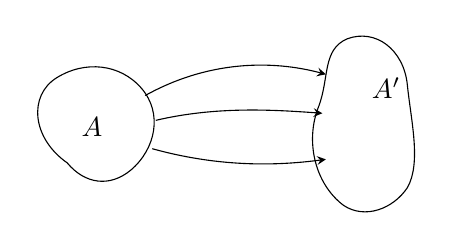
\begin{tikzpicture}[>=stealth,scale=0.9]
  \draw (-2.6,-0.5) .. controls (-3.1,-0.15) and (-3.15,0.45) .. (-2.75,0.7)
        .. controls (-2.35,0.95) and (-1.85,0.9) .. (-1.55,0.55)
        .. controls (-1.25,0.2) and (-1.35,-0.3) .. (-1.7,-0.6)
        .. controls (-2.0,-0.85) and (-2.35,-0.8) .. (-2.6,-0.5);%
  \node at (-2.25,0) {$A$};
  \draw (1.3,-1.1) .. controls (0.9,-0.8) and (0.75,-0.2) .. (0.95,0.3)
        .. controls (1.1,0.7) and (1.0,1.1) .. (1.35,1.25)
        .. controls (1.75,1.4) and (2.15,1.1) .. (2.2,0.6)
        .. controls (2.25,0.1) and (2.4,-0.5) .. (2.2,-0.85)
        .. controls (2.0,-1.15) and (1.6,-1.3) .. (1.3,-1.1);%
  \node at (1.9,0.55) {$A'$};
  \draw[->] (-1.5,0.45) .. controls (-0.6,0.95) and (0.3,0.95) .. (1.05,0.75);%
  \draw[->] (-1.35,0.1) .. controls (-0.5,0.3) and (0.3,0.25) .. (1.0,0.2);%
  \draw[->] (-1.4,-0.3) .. controls (-0.5,-0.55) and (0.3,-0.55) .. (1.05,-0.45);%
\end{tikzpicture}

图 5.3
\end{minipage}

正是这个问题引出了下述由 H.~\trHofer{} [116] 引入的\trDisplacementEnergy{} $e(A)$%
的定义：
\begin{align*}
e(A)\ &=\ \inf\bigl\{\,\lVert H\rVert\ \ \bigm|\ H\in\mathcal{H}\ \text{且}\ \psi_{H}(A)\cap A=\varnothing\ \bigr\}\\
&=\ \inf\bigl\{\,E(\psi)\ \ \bigm|\ \psi\in\mathcal{D}\ \text{且}\ \psi(A)\cap A=\varnothing\ \bigr\}.
\end{align*}
对无界集 $B$ 我们干脆令
\[
e(B)=\sup\bigl\{\,e(A)\ \bigm|\ A\subset B\ \text{且}\ A\ \text{有界}\ \bigr\}.
\]
显然，$e$ 是单调的，其含义是：若 $A\subset B$，则 $e(A)\leq e(B)$。对 $\R^{2n}$ 的%
每个\trSymplecticDiffeomorphism{} $\vartheta$ 都有 $e\bigl(\vartheta(A)\bigr)=e(A)$；%
这由 $E\bigl(\vartheta\circ\psi\circ\vartheta^{-1}\bigr)=E(\psi)$ 推出。此外，对每个%
\trOpenSet{} $U$ 都有 $e(U)>0$。的确，由\cref{thm:energy-dominates-capacity}立即得出%
下述更加定量化的陈述。

\begin{theorem}\label{thm:capacity-le-displacement}
对每个开的 $U$，
\[
c_{0}(U)\ \leq\ e(U).
\]
\end{theorem}

更明确地，我们有估计
\[
\sup\bigl\{\,\lVert H\rVert\ \bigm|\ H\in\mathcal{H}_{a}(U)\bigr\}\ \leq%
\inf\bigl\{\,\lVert H\rVert\ \bigm|\ H\in\mathcal{H},\ \psi_{H}(U)\cap U=\varnothing\bigr\}.
\]

这一估计比乍看之下的样子要强得多。我们将见到，特别地，\trCapacity{} $c_{0}$ 的%
存在性，即 $c_{0}\bigl(B(1)\bigr)=\pi=c_{0}\bigl(Z(1)\bigr)$，是这一估计的直接推论。%
回顾 $c_{0}$ 的这一\trNormalization{}曾是 $c_{0}$ 构造中的微妙之处，该构造需要一个%
存在性证明。我们要指出，\trCapacity{} $c_{0}$ 不仅解释了第 2 章中讨论过的诸%
\trSymplectic\trRigidity{}现象，而且还解释了第 4 章中诸\trPeriodicOrbit{}的存在性现象。

\begin{corollary}\label{cor:ball-cylinder-pi}
对开\trBall{} $B=B(1)$ 与开\trCylinder{} $Z=Z(1)$，我们有
\[
\pi\ \leq\ c_{0}(B)\ \leq\ e(B)\ \leq\ e(Z)\ \leq\ \pi.
\]
\end{corollary}

\begin{proof}
据\cref{thm:capacity-le-displacement}与 $e$ 的单调性，只需证明第一个与最后一个%
不等式。第一个不等式就是第 3 章中的\cref{lem:ball-ge-pi}，它的证明当时需要构造%
一个简单的例子。剩下要证明 $e(Z)\leq\pi$。为此，只需证明对每个半径 $R>1$ 都有
\[
e\bigl(B^{2}(1)\times B^{2n-2}(R)\bigr)\ \leq\ \pi
\]
要把这个集从其自身挪开，只需把 $B^{2}(1)\subset\R^{2}$ 从其自身挪开。为此我们先取%
$\R^{2}$ 的一个保面积且保定向的\trDiffeomorphism{} $\varphi$，它把 $B^{2}(1)$ 映入%
一个边长为 $\sqrt{\pi}+\varepsilon$ 的正方形。

\noindent\begin{minipage}{\linewidth}
\centering
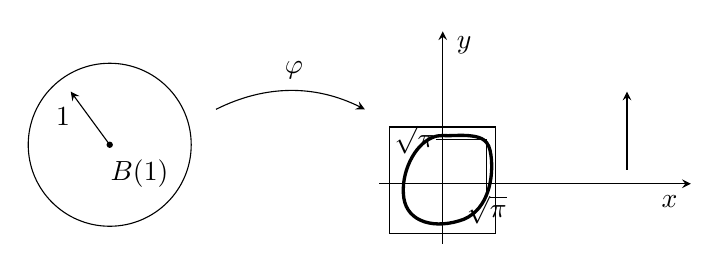
\begin{tikzpicture}[>=stealth,scale=0.9]
  \draw (0,0) circle (1.15);%
  \fill (0,0) circle (0.045);
  \draw[->] (0,0) -- (-0.55,0.75);%
  \node at (-0.66,0.4) {$1$};
  \node at (0.42,-0.4) {$B(1)$};
  \draw[->] (1.5,0.5) .. controls (2.2,0.85) and (2.9,0.85) .. (3.6,0.5);%
  \node at (2.6,1.05) {$\varphi$};
  \draw[->] (4.7,-1.4) -- (4.7,1.6);%
  \node at (5.0,1.4) {$y$};
  \draw[->] (3.8,-0.55) -- (8.2,-0.55);%
  \node at (7.9,-0.8) {$x$};
  \draw (3.95,-1.25) rectangle (5.45,0.25);%
  \draw (4.7,-0.55) rectangle (5.32,0.07);%
  \draw (4.6,0.07) -- (4.8,0.07);%
  \node at (4.3,0.07) {$\sqrt{\pi}$};
  \draw (5.32,-0.65) -- (5.32,-0.45);%
  \node at (5.32,-0.92) {$\sqrt{\pi}$};
  \draw[very thick] (4.85,0.13) .. controls (5.3,0.15) and (5.35,0.05) .. (5.38,-0.15)
        .. controls (5.42,-0.45) and (5.35,-0.9) .. (5.0,-1.05)
        .. controls (4.6,-1.2) and (4.2,-1.1) .. (4.15,-0.75)
        .. controls (4.1,-0.4) and (4.3,0.0) .. (4.55,0.1)
        .. controls (4.65,0.15) and (4.75,0.12) .. (4.85,0.13);%
  \draw[->] (7.3,-0.35) -- (7.3,0.75);%
\end{tikzpicture}

图 5.4
\end{minipage}

一个沿 $y$ 方向、能把该正方形从其自身挪开的\trTranslation{}需要一个斜率接近%
$\sqrt{\pi}$ 的\trHamiltonianFunction，例如%
$H_{1}(x,y)=\bigl(\sqrt{\pi}+2\varepsilon\bigr)\cdot x$。通过把这个%
\trHamiltonianFunction{}光滑地截断，我们便看到：可以用一个\trNorm{} $\lVert H\rVert$%
可任意接近 $\pi$ 的\trHamiltonianFunction{} $H\in\mathcal{H}$ 把该正方形从其自身%
分离出来。于是所要的\trFlow{} $\varphi^{-1}\circ\varphi^{t}\circ\varphi$ 便在时间 1 内把%
$B^{2}(1)$ 从其自身挪开，这就证明了论断，从而证明了该\trhCorollary。
\end{proof}

如图 5.5 所示，这一构造还表明：把一个给定的\trBounded{}集 $V$ 剖分成小的互%
\trDisjoint{}的\trCube，并在去掉一个测度任意小的集 $V_{\varepsilon}\subset V$ 之后，剩下的集%
$V\setminus V_{\varepsilon}$ 便可以用任意小的\trEnergy{}从其自身挪开。

\noindent\begin{minipage}{\linewidth}
\centering
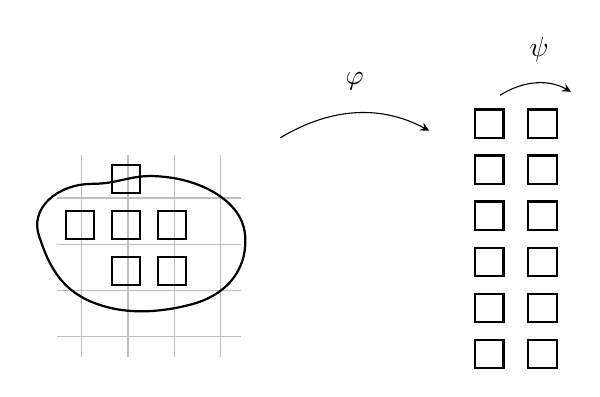
\begin{tikzpicture}[>=stealth,scale=0.9]
  \draw[black!25] (0.3,-1.6) grid[step=0.65] (2.9,1.25);%
  \draw[thick] (0.05,0.1) .. controls (-0.1,0.5) and (0.3,0.85) .. (0.8,0.85)
        .. controls (1.2,0.85) and (1.35,1.0) .. (1.8,0.95)
        .. controls (2.35,0.9) and (2.9,0.6) .. (2.95,0.15)
        .. controls (3.0,-0.3) and (2.75,-0.7) .. (2.2,-0.85)
        .. controls (1.7,-0.98) and (1.2,-1.0) .. (0.75,-0.8)
        .. controls (0.35,-0.62) and (0.18,-0.3) .. (0.05,0.1);%
  \draw[thick] (1.07,0.72) rectangle (1.47,1.12);%
  \draw[thick] (0.42,0.07) rectangle (0.82,0.47);%
  \draw[thick] (1.07,0.07) rectangle (1.47,0.47);%
  \draw[thick] (1.72,0.07) rectangle (2.12,0.47);%
  \draw[thick] (1.07,-0.58) rectangle (1.47,-0.18);%
  \draw[thick] (1.72,-0.58) rectangle (2.12,-0.18);%
  \draw[->] (3.45,1.5) .. controls (4.2,1.95) and (4.9,1.95) .. (5.55,1.6);%
  \node at (4.5,2.3) {$\varphi$};
  \foreach \y in {1.5,0.85,0.2,-0.45,-1.1,-1.75}{%
    \draw[thick] (6.2,\y) rectangle (6.6,\y+0.4);
    \draw[thick] (6.95,\y) rectangle (7.35,\y+0.4);}
  \draw[->] (6.55,2.1) .. controls (6.9,2.32) and (7.25,2.32) .. (7.55,2.15);%
  \node at (7.1,2.75) {$\psi$};
\end{tikzpicture}

图 5.5
\end{minipage}

\begin{definition}\label{def:special-capacity}
$\R^{2n}$ 中开集的\textbf{\trSpecialCapacity}（special capacity）$c$ 是一个映射 $c$，它对%
开集 $U$ 配上一个数 $c(U)$ 或 $+\infty$，使得

\textbf{(A.1)}\ 若 $U\neq\varnothing$，则 $c(U)>0$，且%
$c\bigl(B^{2}(1)\times\R^{2n-2}\bigr)<\infty$。

\textbf{(A.2)}\ 若 $\psi:\R^{2n}\to\R^{2n}$ 是一个\trDiffeomorphism{}且满足%
$\psi^{*}\omega=\alpha\omega$（$\alpha\neq0$ 为某一常数）与 $\psi(U)\subset V$，%
则 $\lvert\alpha\rvert\,c(U)\leq c(V)$。
\end{definition}

显然，每个\trCapacity{}都是一个\trSpecialCapacity。然而，与第 2 章\trCapacity{}的诸公理%
相反，(A.2) 中的诸映射 $\psi$ 要求定义在整个 $\R^{2n}$ 上。

\begin{theorem}\label{thm:displacement-special-capacity}
\trDisplacementEnergy{} $e$ 是 $\R^{2n}$ 中的一个\trSpecialCapacity，并且它还满足%
$e\bigl(B(1)\bigr)=\pi=e\bigl(Z(1)\bigr)$。
\end{theorem}

\begin{proof}
余下的只需证明 $e$ 满足 (A.2)。设 $\psi$ 满足 $\psi^{*}\omega=\alpha\omega$，则对%
$\varphi\in\mathcal{D}$ 有 $E\bigl(\psi\varphi\psi^{-1}\bigr)=\lvert\alpha\rvert E(\varphi)$。%
若 $\varphi(U)\cap U=\varnothing$，则%
$\psi\varphi\psi^{-1}\bigl(\psi(U)\bigr)\cap\psi(U)=\varnothing$，这蕴含%
$e\bigl(\psi(U)\bigr)=\lvert\alpha\rvert e(U)$。现在若 $U\subset V$，则%
$e(U)\leq e(V)$，于是 $\psi(U)\subset V$ 便蕴含%
$e\bigl(\psi(U)\bigr)=\lvert\alpha\rvert e(U)\leq e(V)$，正是所要证的。
\end{proof}

应当指出，$e$ 并不是第 2 章中所定义的那类\trCapacity，而且 $c_{0}\neq e$。的确，%
考察 $\R^{2}$ 中的一个\trAnnulus{} $A$。

则 $c_{0}(A)=\pi\bigl(R^{2}-r^{2}\bigr)$，亦即它是 $A$ 的面积。若%
$\psi\in\mathcal{D}$（按定义，它定义在整个 $\R^{2}$ 上）满足%
$\psi(A)\cap A=\varnothing$，则必有 $\psi\bigl(B(R)\bigr)\cap B(R)=\varnothing$。%
利用 $\psi$ 为保面积映射这一事实，此结论由拓扑上的理由可得，于是我们见到
\[
e(A)=e\bigl(B(R)\bigr)=\pi R^{2}>c_{0}(A).
\]

\noindent\begin{minipage}{\linewidth}
\centering
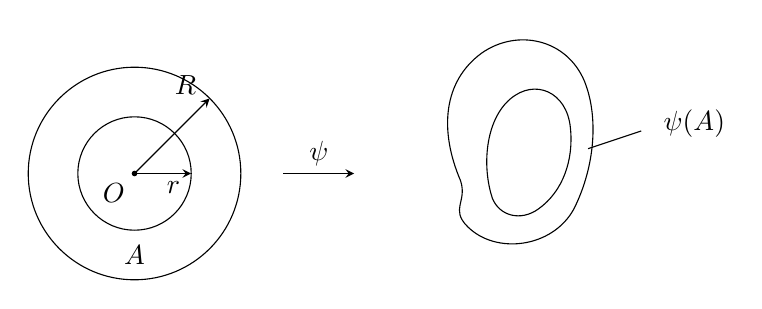
\begin{tikzpicture}[>=stealth,scale=0.9]
  \fill (0,0) circle (0.04);%
  \node[below left] at (0,0) {$O$};
  \draw (0,0) circle (1.5);%
  \draw (0,0) circle (0.8);%
  \draw[->] (0,0) -- (1.06,1.06);%
  \node at (0.72,1.25) {$R$};
  \draw[->] (0,0) -- (0.8,0);%
  \node at (0.55,-0.2) {$r$};
  \node at (0,-1.15) {$A$};
  \draw[->] (2.1,0) -- (3.1,0);%
  \node at (2.6,0.28) {$\psi$};
  \draw (4.6,-0.1) .. controls (4.3,0.6) and (4.35,1.3) .. (4.9,1.7)
        .. controls (5.4,2.05) and (6.1,1.9) .. (6.35,1.3)
        .. controls (6.55,0.8) and (6.5,0.1) .. (6.2,-0.5)
        .. controls (5.9,-1.05) and (5.1,-1.15) .. (4.7,-0.75)
        .. controls (4.45,-0.5) and (4.7,-0.4) .. (4.6,-0.1);%
  \draw (5.05,-0.35) .. controls (4.9,0.1) and (4.95,0.75) .. (5.3,1.05)
        .. controls (5.65,1.35) and (6.1,1.15) .. (6.15,0.65)
        .. controls (6.2,0.2) and (6.05,-0.25) .. (5.7,-0.5)
        .. controls (5.45,-0.68) and (5.15,-0.6) .. (5.05,-0.35);%
  \draw (6.4,0.35) -- (7.15,0.6);%
  \node at (7.9,0.7) {$\psi(A)$};
\end{tikzpicture}

图 5.6
\end{minipage}
\par
